\documentclass[a4paper,twoside]{article}
\usepackage[T1]{fontenc}
\usepackage[bahasa]{babel}
\usepackage{graphicx}
\usepackage{graphics}
\usepackage{float}
\usepackage[cm]{fullpage}
\pagestyle{myheadings}
\usepackage{etoolbox}
\usepackage{setspace} 
\usepackage{lipsum} 
\setlength{\headsep}{30pt}
\usepackage[inner=2cm,outer=2.5cm,top=2.5cm,bottom=2cm]{geometry} %margin
% \pagestyle{empty}

\makeatletter
\renewcommand{\@maketitle} {\begin{center} {\LARGE \textbf{ \textsc{\@title}} \par} \bigskip {\large \textbf{\textsc{\@author}} }\end{center} }
\renewcommand{\thispagestyle}[1]{}
\markright{\textbf{\textsc{Laporan Perkembangan Pengerjaan Skripsi\textemdash Sem. Ganjil 2017/2018}}}

\onehalfspacing
 
\begin{document}

\title{\@judultopik}
\author{\nama \textendash \@npm} 

%ISILAH DATA BERIKUT INI:
\newcommand{\nama}{Gavrila Tiominar Sianturi}
\newcommand{\@npm}{2013730025}
\newcommand{\tanggal}{28/11/2017} %Tanggal pembuatan dokumen
\newcommand{\@judultopik}{Steganografi dengan Teknik Indikasi Piksel} % Judul/topik anda
\newcommand{\kodetopik}{MTA4304*}
\newcommand{\jumpemb}{1} % Jumlah pembimbing, 1 atau 2
\newcommand{\pembA}{Mariskha Tri Adithia}
\newcommand{\pembB}{-}
\newcommand{\semesterPertama}{43 - Ganjil 17/18} % semester pertama kali topik diambil, angka 1 dimulai dari sem Ganjil 96/97
\newcommand{\lamaSkripsi}{1} % Jumlah semester untuk mengerjakan skripsi s.d. dokumen ini dibuat
\newcommand{\kulPertama}{Skripsi 1} % Kuliah dimana topik ini diambil pertama kali
\newcommand{\tipePR}{B} % tipe progress report :
% A : dokumen pendukung untuk pengambilan ke-2 di Skripsi 1
% B : dokumen untuk reviewer pada presentasi dan review Skripsi 1
% C : dokumen pendukung untuk pengambilan ke-2 di Skripsi 2

% Dokumen hasil template ini harus dicetak bolak-balik !!!!

\maketitle

\pagenumbering{arabic}

\section{Data Skripsi} %TIDAK PERLU MENGUBAH BAGIAN INI !!!
Pembimbing utama/tunggal: {\bf \pembA}\\
Pembimbing pendamping: {\bf \pembB}\\
Kode Topik : {\bf \kodetopik}\\
Topik ini sudah dikerjakan selama : {\bf \lamaSkripsi} semester\\
Pengambilan pertama kali topik ini pada : Semester {\bf \semesterPertama} \\
Pengambilan pertama kali topik ini di kuliah : {\bf \kulPertama} \\
Tipe Laporan : {\bf \tipePR} -
\ifdefstring{\tipePR}{A}{
			Dokumen pendukung untuk {\BF pengambilan ke-2 di Skripsi 1} }
		{
		\ifdefstring{\tipePR}{B} {
				Dokumen untuk reviewer pada presentasi dan {\bf review Skripsi 1}}
			{	Dokumen pendukung untuk {\bf pengambilan ke-2 di Skripsi 2}}
		}

\section{Detail Perkembangan Pengerjaan Skripsi}
Detail bagian pekerjaan skripsi sesuai dengan rencan kerja/laporan perkembangan terkahir :
	\begin{enumerate}
		\item \textbf{Melakukan studi literatur mengenai dasar-dasar steganografi, metode steganografi dengan teknik indikasi piksel, dan metode steganografi dengan algoritma \textit{Triple-A}}\\
		{\bf Status :} Diganti (metode \textit{Triple-A} diganti menjadi metode \textit{Least Significant Bit}).\\
		{\bf Hasil :} Berikut merupakan hasil studi literatur mengenai dasar-dasar steganografi, steganografi dengan teknik \textit{Least Significant Bit}, dan steganografi dengan teknik indikasi piksel. 
		
		\begin{itemize}
		\item \textbf{Steganografi}\\
		Steganografi merupakan seni dan ilmu untuk menyembunyikan pesan rahasia (\textit{secret data}) di dalam suatu \textit{cover media}. Kata steganografi berasal dari bahasa Yunani yang berarti tulisan yang tersembunyi. Tujuan dilakukannya steganografi adalah untuk mengirimkan pesan rahasia melalui suatu media, dimana media tersebut dapat dikirimkan melalui apapun dan diterima oleh siapa saja, tanpa menimbulkan kecurigaan bahwa ada pesan rahasia yang disembunyikan di dalamnya.\\
		
		Steganografi dapat dilakukan dengan menggunakan berbagai media. Media yang dapat digunakan antara lain adalah audio, video, gambar, teks, dan lain sebagainya. Media steganografi yang akan digunakan pada skripsi ini adalah gambar, dimana informasi rahasia akan disembunyikan ke dalam piksel-piksel pada gambar. Hasil dari implementasi steganografi akan berupa gambar yang di dalam piksel-pikselnya terdapat informasi rahasia. Gambar hasil implementasi steganografi disebut \textit{stego image}. Gambar \ref{fig:imagestegano} memperlihatkan alur proses implementasi steganografi dengan media gambar. \textit{Secret data} dan \textit{cover media} (atau yang dapat juga disebut \textit{cover image}) akan diproses oleh algoritma steganografi dan proses tersebut akan menghasilkan \textit{stego image}.\\
		
		\begin{figure}[!htbp]
		\centering
		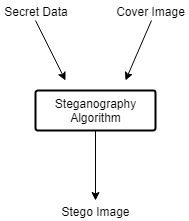
\includegraphics[scale=0.7]{Embedding.png}
		\caption{Steganografi dengan media gambar}
		\label{fig:imagestegano}
		\end{figure} 
		
		Steganografi dengan media gambar melibatkan beberapa aspek untuk dipertimbangkan. Berikut merupakan beberapa aspek diantaranya yang akan digunakan pada skripsi ini.
		\begin{itemize}		
		\item Kapasitas (\textit{capacity})\\
		Kapasitas merupakan jumlah data yang dapat disembunyikan pada gambar tanpa mengubah gambar tersebut secara signifikan.
		\item Transparansi (\textit{invisibility})\\
		Transparansi berarti hasil dari proses penyembunyian tidak menimbulkan kecurigaan bagi pihak yang tidak berkepentingan.	
		\item Keamanan (\textit{security})\\
		Keamanan berarti \textit{secret data} tidak bisa didapatkan dengan mudah oleh pihak-pihak yang tidak berkepentingan.
		\end{itemize}
		
		Aspek-aspek tersebut digunakan sebagai ukuran pembanding berbagai metode steganografi. Aspek-aspek ini berpengaruh satu sama lain, seperti apabila kapasitas bertambah maka ada kemungkinan transparansi akan berkurang karena akan semakin banyak nilai piksel yang diganti.\\
		
		Pada skripsi ini, \textit{cover media} yang digunakan untuk menyembunyikan \textit{secret data} berupa gambar berwarna atau gambar RGB. Setiap piksel pada gambar RGB terdiri dari tiga \textit{channel} warna, yaitu merah, hijau, dan biru. Nilai setiap \textit{channel} warna pada setiap piksel direpresentasikan dengan 8 bit angka biner, sehingga setiap piksel direpresentasikan dengan 24 bit angka biner.\\
		
		\item \textbf{Steganografi dengan Teknik \textit{Least Significant Bit}}\\
		Steganografi dengan metode \textit{Least Significant Bit} (LSB) merupakan salah satu metode yang sudah banyak digunakan karena implementasinya yang tergolong sederhana. Penyembunyian \textit{secret data} di dalam \textit{cover media} dilakukan dengan cara menyisipkan \textit{secret data}, yang sudah diubah ke dalam bentuk 8 bit angka biner ASCII, ke setiap satu bit terakhir setiap \textit{channel} warna pada setiap piksel. Sebagai contoh, \textit{secret data} yang ingin disembunyikan adalah A. Karakter A apabila diubah dalam bentuk biner ASCII adalah 01000001. Piksel \textit{cover media} yang digunakan adalah:
		
		\begin{center}
		00100111 11101001 11001000\\
		00100111 11001000 11101001\\
		11001000 00100111 11101001
		\end{center}
		
		Maka, hasil piksel setelah diimplementasikan steganografi dengan teknik LSB adalah:
		
		\begin{center}
		0010011\underline{0} 1110100\underline{1} 1100100\underline{0}\\
		0010011\underline{0} 1100100\underline{0} 111010\underline{0}\\
		1100100\underline{0} 0010011\underline{1} 11101001
		\end{center}
		
		Penyisipan \textit{secret data} dilakukan pada bit terakhir setiap \textit{channel} warna dengan tujuan supaya perubahan nilai warna pada piksel tidak besar sehingga tidak menunjukkan perbedaan yang signifikan antara \textit{cover media} yang asli dengan \textit{cover media} yang sudah disisipkan \textit{secret data}.\\
		
		\item \textbf{Steganografi dengan Teknik Indikasi Piksel}\\
		Steganografi dengan teknik indikasi piksel merupakan metode pengembangan dari teknik LSB. Sama seperti LSB, \textit{secret data} diubah terlebih dahulu ke dalam bentuk biner ASCII. Bit-bit \textit{secret data} juga tetap disembunyikan pada bit terakhir suatu \textit{channel} warna, namun tidak semua \textit{channel} warna pasti dipakai untuk menyembunyikan \textit{secret data}. Salah satu \textit{channel} warna akan digunakan sebagai indikator untuk menentukan penyisipan bit \textit{secret data} pada \textit{channel} warna lainnya.\\
		
		Langkah pertama yang dilakukan dalam implementasi teknik indikasi piksel adalah menghitung panjang karakter \textit{secret data}. Panjang karakter tersebut akan diubah dalam bentuk 8 bit angka biner dan disisipkan ke dalam bit terakhir pada 8 byte piksel pertama \textit{cover media}. Penyisipan bit \textit{secret data} akan dimulai pada baris piksel yang selanjutnya, sehingga akan tersisa satu \textit{channel} warna pada piksel akhir penyisipan panjang \textit{secret data} yang tidak disisipkan apapun.\\
		
		 Langkah selanjutnya dalam implementasi teknik indikasi piksel adalah menentukan \textit{channel} warna yang menjadi indikator. \textit{Channel} warna yang menjadi indikator dipilih berdasarkan panjang karakter \textit{secret data}. Apabila panjang \textit{secret data} merupakan bilangan genap, maka \textit{channel} warna yang menjadi indikator adalah merah. Apabila panjang \textit{secret data} merupakan bilangan prima, maka \textit{channel} warna yang menjadi indikator adalah biru. Apabila panjang \textit{secret data} bukan bilangan genap atau prima, maka \textit{channel} warna yang akan menjadi indikator adalah hijau.\\
		 
		Panjang \textit{secret data} juga akan digunakan untuk menentukan warna yang menjadi \textit{channel} 1 dan \textit{channel} 2 dalam penyisipan bit \textit{secret data}. Panjang \textit{secret data} akan diubah ke dalam bentuk biner untuk menentukan apakah panjang \textit{secret data} tersebut termasuk \textit{odd parity} atau \textit{even parity}. Apabila jumlah bit 1 pada biner panjang \textit{secret data} berjumlah ganjil, maka \textit{channel} 1 dan 2 ditentukan berdasarkan kolom \textit{odd parity}. Sebaliknya, apabila jumlah bit 1 pada biner panjang \textit{secret data} berjumlah genap, maka \textit{channel} 1 dan 2 ditentukan berdasarkan kolom \textit{even parity}. Tabel \ref{tabelIndSel} memperlihatkan ketentuan yang digunakan untuk menentukan \textit{channel} indikator, \textit{channel} 1, dan \textit{channel} 2 yang digunakan untuk menyisipkan \textit{secret data}.\\
		
		\begin{table}[!htbp]
		\centering
		\caption{Tabel kriteria pemilihan indikator \textit{channel} warna} 
		\label{tabelIndSel}
		\begin{tabular}{| c | c | c | c |}
		\hline
		Tipe panjang \textit{secret data} (N) & Pemilihan \textit{channel} indikator & \multicolumn{2}{|c|}{Pemilihan \textit{channel} 1 dan 2}\\\cline{3-4}
		& & Odd parity & Even Parity\\
		\hline
		Genap & R & GB & BG\\
		\hline
		Prima & B & RG & GR\\
		\hline
		Lainnya & G & RB & BR\\
		\hline		
		\end{tabular}
		\end{table}
		
		Setelah ditetapkan \textit{channel} warna yang menjadi indikator, \textit{channel} 1, dan \textit{channel} 2, langkah yang harus dilakukan adalah menyisipkan bit-bit \textit{secret data} berdasarkan nilai \textit{channel} warna indikator pada piksel tersebut. Nilai \textit{channel} warna direpresentasikan dalam 8 bit angka biner. Dua bit terakhir nilai \textit{channel} warna indikator digunakan untuk menentukan jumlah dan posisi penyisipan bit-bit \textit{secret data} pada suatu piksel. Apabila dua bit terakhir pada nilai \textit{channel} warna adalah 00, maka tidak ada bit \textit{secret data} yang disembunyikan dalam \textit{channel} 1 dan 2 pada piksel tersebut. Apabila dua bit terakhir pada nilai \textit{channel} warna indikator adalah 01, maka tidak ada bit \textit{secret data} yang disembunyikan dalam \textit{channel} 1 piksel tersebut dan ada 2 bit data yang disembunyikan dalam \textit{channel} 2 piksel tersebut. Apabila dua bit terakhir pada nilai \textit{channel} warna indikator adalah 10, maka ada 2 bit data yang disembunyikan dalam \textit{channel} 1 piksel tersebut dan tidak ada bit \textit{secret data} yang disembunyikan dalam \textit{channel} 2 piksel tersebut. Apabila dua bit terakhir pada nilai \textit{channel} warna indikator adalah 11, maka ada 2 bit data yang disembunyikan dalam \textit{channel} 1 piksel tersebut dan ada 2 bit data yang disembunyikan dalam \textit{channel} 2 piksel tersebut. Tabel \ref{tabelIndAct} memperlihatkan bagaimana data akan disisipkan dalam satu piksel berdasarkan dua bit terakhir nilai \textit{channel} warna yang menjadi indikator.\\
		
		\begin{table}[!htbp]
		\centering
		\caption{Tabel kriteria pemilihan indikator \textit{channel} warna} 
		\label{tabelIndAct}
		\begin{tabular}{| c | c | c |}
		\hline
		\textit{Channel} indikator & \textit{Channel} 1 & \textit{Channel} 2\\
		\hline
		00 & Tidak ada data yang disisipkan & Tidak ada data yang disisipkan\\
		\hline
		01 & Tidak ada data yang disisipkan & Disisipkan 2 bit data\\
		\hline
		10 & Disisipkan 2 bit data & Tidak ada data yang disisipkan\\
		\hline
		11 & Disisipkan 2 bit data & Disisipkan 2 bit data\\
		\hline
		\end{tabular}
		\end{table}	
			
		Penyisipan bit-bit \textit{secret data} dilakukan dengan menggunakan iterasi. Dalam satu piksel dapat disisipkan 0 sampai 4 bit \textit{secret data} yang ditentukan berdasarkan nilai \textit{channel} indikator. Oleh karena penyisipan bit-bit \textit{secret data} dilakukan secara iterasi, maka dibutuhkan suatu variabel untuk menentukan kondisi berhenti iterasi tersebut. Variabel \textit{Remaining Message Size} (RMS) digunakan untuk menentukan kondisi berhenti dengan memeriksa apakah seluruh bit \textit{secret data} sudah disisipkan pada \textit{cover media} atau belum. Variabel RMS pada awalnya diinisialisasi dengan jumlah bit \textit{secret data} yang akan disisipkan. Setiap iterasi penyisipan bit-bit \textit{secret data} pada piksel, variabel RMS akan dikurangi dengan jumlah bit \textit{secret data} yang disisipkan pada piksel tersebut. Iterasi penyisipan akan berhenti ketika variabel RMS sudah bernilai 0, dimana seluruh bit \textit{secret data} sudah disisipkan.\\	
		
		\begin{figure}[!htbp]
		\centering
		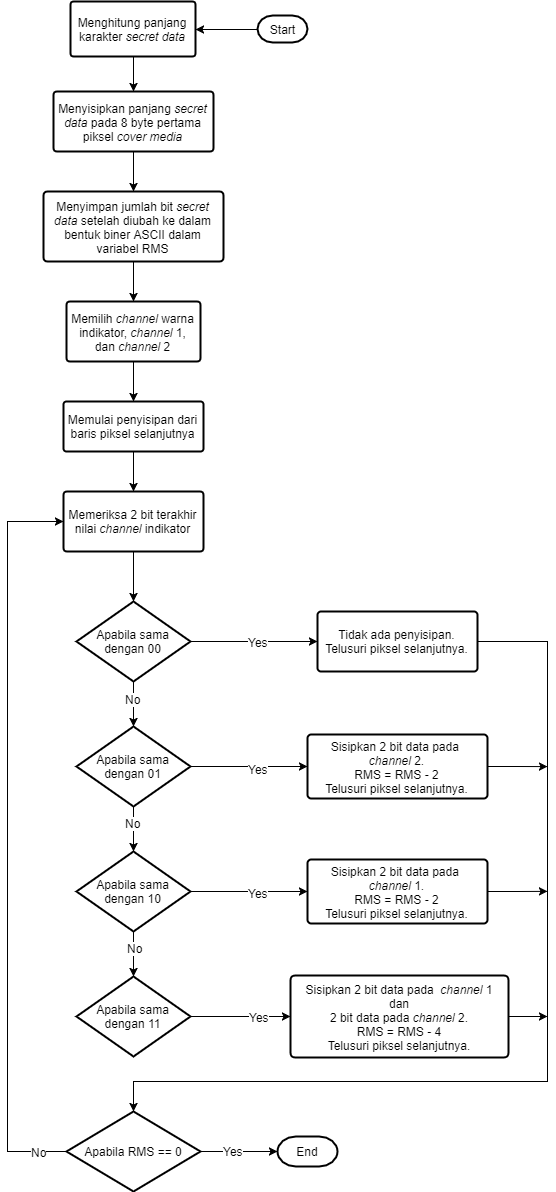
\includegraphics[scale=0.5]{PIT.png}
		\caption{Algoritma implementasi teknik indikasi piksel}
		\label{imagePIT}
		\end{figure}
			
		Gambar \ref{imagePIT} memperlihatkan cara implementasi teknik indikasi piksel secara keseluruhan. Berikut merupakan penjelasan setiap langkah yang terdapat pada ilustrasi teknik indikasi piksel dalam Gambar \ref{imagePIT}.		
		\begin{itemize}
			\item Menghitung panjang karakter \textit{secret data}\\
			Panjang \textit{secret data} dihitung per karakter.
			\item Menyisipkan panjang \textit{secret data} pada 8 byte pertama piksel \textit{cover media}\\
			Panjang \textit{secret data} diubah ke dalam bentuk 8 bit angka biner kemudian disisipkan dalam bit terakhir 8 byte pertama piksel \textit{cover media}.
			\item Menyimpan jumlah bit \textit{secret data} setelah diubah ke dalam bentuk biner ASCII dalam variabel RMS\\
			\textit{Secret data} diubah ke dalam bentuk biner ASCII. Masing-masing karakter direpresentasikan dalam 8 bit angka biner. Jumlah seluruh bit bentuk ASCII \textit{secret data} dimasukkan ke dalam variabel RMS.
			\item Memilih \textit{channel} warna indikator, \textit{channel} 1, dan \textit{channel} 2\\
			Memilih \textit{channel} warna yang menjadi indikator, \textit{channel} 1, dan \textit{channel} 2 berdasarkan panjang \textit{secret data}. \textit{Channel} indikator, \textit{channel} 1, dan \textit{channel} 2 dipilih berdasarkan ketentuan pada Tabel \ref{tabelIndSel}.
			\item Memeriksa 2 bit terakhir nilai \textit{channel} indikator\\
			Melakukan penyisipan bit \textit{secret data} berdasarkan dua bit terakhir nilai \textit{channel} indikator. Berikut merupakan proses yang dilakukan berdasarkan dua bit terakhir nilai \textit{channel} indikator.
			\begin{itemize}
				\item Apabila bernilai 00, tidak akan ada perubahan maka akan langsung dilakukan penelusuran piksel selanjutnya apabila variabel RMS belum bernilai 0. Apabila variabel RMS sudah bernilai 0, maka iterasi akan berhenti.
				\item Apabila bernilai 01, dilakukan penyisipan 2 bit \textit{secret data} pada 2 bit terakhir \textit{channel} 2. Kemudian variabel RMS akan dikurangi dengan 2 karena pada piksel tersebut terdapat 2 bit \textit{secret data} yang disembunyikan. Setelah itu, dilakukan penelusuran piksel selanjutnya apabila variabel RMS belum bernilai 0. Apabila variabel RMS sudah bernilai 0, maka iterasi akan berhenti.
				\item Apabila bernilai 10, dilakukan penyisipan 2 bit \textit{secret data} pada 2 bit terakhir \textit{channel} 1. Kemudian variabel RMS akan dikurangi dengan 2 karena pada piksel tersebut terdapat 2 bit \textit{secret data} yang disembunyikan. Setelah itu, dilakukan penelusuran piksel selanjutnya apabila variabel RMS belum bernilai 0. Apabila variabel RMS sudah bernilai 0, maka iterasi akan berhenti.
				\item Apabila bernilai 11, dilakukan penyisipan 2 bit \textit{secret data} pada 2 bit terakhir \textit{channel} 1 dan 2 bit \textit{secret data} pada 2 bit terakhir \textit{channel} 2. Kemudian variabel RMS akan dikurangi dengan 4 karena pada piksel tersebut terdapat 4 bit \textit{secret data} yang disembunyikan. Setelah itu, dilakukan penelusuran piksel selanjutnya apabila variabel RMS belum bernilai 0. Apabila variabel RMS sudah bernilai 0, maka iterasi akan berhenti.\\
			\end{itemize}		
		\end{itemize}		
		\end{itemize}				
		
		\item \textbf{Mengimplementasikan teknik indikasi piksel dan algoritma \textit{Triple-A} secara manual}\\
		{\bf Status :} Diganti (metode \textit{Triple-A} diganti menjadi metode \textit{Least Significant Bit}).\\
		{\bf Hasil :} Berikut merupakan contoh implementasi manual steganografi dengan teknik LSB dan teknik indikasi piksel.\\
		
		\textit{Secret data} : HELLO\\
		Panjang \textit{secret data} (N) : 5\\
		Contoh nilai-nilai setiap \textit{channel} warna pada piksel-piksel \textit{cover media} diperlihatkan pada Tabel \ref{tabelNilaiPiksel}.\\
		
		\begin{table}[!htbp]
		\centering
		\caption{Tabel nilai piksel pada \textit{cover media}} 
		\label{tabelNilaiPiksel}
		\begin{tabular}{| c | c | c |}
		\hline
		R & G & B\\
		\hline
		00100000 & 01011101 & 10100011\\
		\hline
		00111111 & 01011101 & 10011011\\
		\hline
		00100001 & 01011110 & 10100001\\
		\hline
		00100010 & 01011101 & 10011010\\
		\hline
		00100101 & 01011111 & 10011011\\
		\hline
		00100111 & 01100001 & 10100011\\
		\hline
		00101000 & 01100001 & 10100110\\
		\hline
		00100101 & 01100000 & 10100011\\
		\hline
		00100111 & 01100011 & 10100010\\
		\hline
		00101001 & 01100110 & 10100111\\
		\hline
		00101101 & 01101000 & 10101011\\
		\hline
		00110011 & 01101110 & 10110010\\
		\hline
		00110001 & 01101011 & 10110001\\
		\hline
		00110001 & 01100010 & 10110011\\
		\hline
		00110110 & 01010010 & 10011011\\
		\hline
		00101000 & 01010110 & 10011001\\
		\hline
		00101010 & 01010110 & 10010100\\
		\hline
		00100010 & 01000010 & 10010001\\
		\hline
		00110101 & 01000110 & 10010111\\
		\hline
		\end{tabular}
		\end{table} 	
			
		Langkah pertama yang dilakukan untuk mengimplementasikan kedua metode steganografi ini adalah dengan mengubah \textit{secret data} ke dalam bentuk biner ASCII. Setiap karakter diubah ke dalam bentuk 8 bit biner ASCII. Pada contoh ini, kata "HELLO" apabila diterjemahkan ke dalam bentuk biner ASCII menjadi 01001000 01000101 01001100 01001100 01001111. Setiap karakter pada \textit{secret data} diubah dalam bentuk biner ASCII supaya dapat disisipkan ke dalam nilai-nilai piksel yang juga berupa angka biner.\\
		
		\begin{itemize}
		\item \textbf{Implementasi dengan Teknik LSB}\\
		Penyisipan dengan metode LSB dilakukan dengan mengganti setiap satu bit terakhir pada setiap \textit{channel} warna dalam setiap piksel dengan satu bit \textit{secret data} secara berurutan. Tabel \ref{TabelLSB} menunjukkan perubahan nilai piksel hasil implementasi steganografi dengan teknik LSB.\\
		
		\begin{table}[!htbp]				
		\centering		
		\caption{Tabel perbandingan nilai piksel awal dan nilai piksel setelah disisipkan bit \textit{secret data} dengan metode LSB}
		\label{TabelLSB}
		\begin{tabular}{| c | c | c |}
		\hline
		R & G & B\\
		\hline
		00100000 & 01011101 & 10100011\\
		\hline
		00111111 & 01011101 & 10011011\\
		\hline
		00100001 & 01011110 & 10100001\\
		\hline
		00100010 & 01011101 & 10011010\\
		\hline
		00100101 & 01011111 & 10011011\\
		\hline
		00100111 & 01100001 & 10100011\\
		\hline
		00101000 & 01100001 & 10100110\\
		\hline
		00100101 & 01100000 & 10100011\\
		\hline
		00100111 & 01100011 & 10100010\\
		\hline
		00101001 & 01100110 & 10100111\\
		\hline
		00101101 & 01101000 & 10101011\\
		\hline
		00110011 & 01101110 & 10110010\\
		\hline
		00110001 & 01101011 & 10110001\\
		\hline
		00110001 & 01100010 & 10110011\\
		\hline
		00110110 & 01010010 & 10011011\\
		\hline
		00101000 & 01010110 & 10011001\\
		\hline
		00101010 & 01010110 & 10010100\\
		\hline
		00100010 & 01000010 & 10010001\\
		\hline
		00110101 & 01000110 & 10010111\\
		\hline
		\end{tabular}
		\quad
		\begin{tabular}{| c | c | c |}
		\hline
		R & G & B\\
		\hline
		0010000\underline{0} & 0101110\underline{1} & 1010001\underline{0}\\
		\hline
		0011111\underline{0} & 0101110\underline{1} & 1001101\underline{0}\\
		\hline
		0010000\underline{0} & 0101111\underline{0} & 1010000\underline{0}\\
		\hline
		0010001\underline{1} & 0101110\underline{0} & 1001101\underline{0}\\
		\hline
		0010010\underline{0} & 0101111\underline{1} & 1001101\underline{0}\\
		\hline
		0010011\underline{1} & 0110000\underline{0} & 1010001\underline{1}\\
		\hline
		0010100\underline{0} & 0110000\underline{0} & 1010011\underline{1}\\
		\hline
		0010010\underline{1} & 0110000\underline{0} & 1010001\underline{0}\\
		\hline
		0010011\underline{0} & 0110001\underline{1} & 1010001\underline{0}\\
		\hline
		0010100\underline{0} & 0110011\underline{1} & 1010011\underline{1}\\
		\hline
		0010110\underline{0} & 0110100\underline{0} & 1010101\underline{0}\\
		\hline
		0011001\underline{1} & 0110111\underline{0} & 1011001\underline{0}\\
		\hline
		0011000\underline{1} & 0110101\underline{1} & 1011000\underline{1}\\
		\hline
		0011000\underline{1} & 01100010 & 10110011\\
		\hline
		00110110 & 01010010 & 10011011\\
		\hline
		00101000 & 01010110 & 10011001\\
		\hline
		00101010 & 01010110 & 10010100\\
		\hline
		00100010 & 01000010 & 10010001\\
		\hline
		00110101 & 01000110 & 10010111\\
		\hline
		\end{tabular}		
		\end{table}
		
		\item \textbf{Implementasi dengan Teknik Indikasi Piksel}\\
		Langkah pertama yang dilakukan pada implementasi teknik indikasi piksel adalah menyimpan panjang \textit{secret data}. Panjang \textit{secret data} akan disimpan dalam 8 bit angka biner karena panjang \textit{secret data} akan disimpan pada setiap bit terakhir 8 byte piksel pertama pada \textit{cover media}. Pada contoh ini, panjang \textit{secret data} adalah 5 karakter, dalam bentuk binernya 00000101. Tabel \ref{TabelStoreSize} memperlihatkan hasil penyisipan panjang \textit{secret data} pada 8 byte pertama piksel \textit{cover media}.\\
		
		\begin{table}[!htbp]
		\centering
		\caption{Tabel perbandingan nilai piksel awal dan nilai piksel setelah disisipkan panjang \textit{secret data}}
		\label{TabelStoreSize}
		\begin{tabular}{| c | c | c |}
		\hline
		R & G & B\\
		\hline
		0010000\textbf{0} & 0101110\textbf{0} & 1010001\textbf{0}\\
		\hline
		0011111\textbf{0} & 0101110\textbf{0} & 1001101\textbf{1}\\
		\hline
		0010000\textbf{0} & 0101111\textbf{1} & 10100001\\
		\hline
		\end{tabular}
		\quad
		\begin{tabular}{| c | c | c |}
		\hline
		R & G & B\\
		\hline
		00100000 & 01011101 & 10100011\\
		\hline
		00111111 & 01011101 & 10011011\\
		\hline
		00100001 & 01011110 & 10100001\\
		\hline
		\end{tabular}		
		\end{table}
		
		Langkah kedua dalam implementasi teknik indikasi piksel adalah menentukan \textit{channel} warna yang menjadi indikator. Dua bit terakhir nilai \textit{channel} warna indikator pada suatu piksel menjadi penentu letak penyisipan bit \textit{secret data} pada piksel tersebut. \textit{Channel} warna yang menjadi indikator dipilih berdasarkan panjang \textit{secret data}. Ketentuan pemilihan \textit{channel} warna yang menjadi indikator terdapat pada Tabel \ref{tabelIndSel}. Pada contoh ini, panjang \textit{secret data} adalah 5. Oleh karena 5 adalah bilangan prima, maka \textit{channel} warna yang menjadi indikator adalah biru.\\
		
		Setelah ditentukan \textit{channel} warna yang menjadi indikator, selanjutnya adalah menentukan \textit{channel} warna mana yang menjadi \textit{channel} 1 dan 2. Pada \textit{channel} 1 dan 2 akan disisipkan bit \textit{secret data} berdasarkan nilai pada \textit{channel} warna indikator. Pemilihan \textit{channel} 1 dan 2 ditentukan berdasarkan apakah panjang \textit{secret data} (dalam bentuk biner) termasuk \textit{odd} atau \textit{even parity}. Panjang \textit{secret data} termasuk \textit{odd parity} apabila jumlah bit 1 pada binernya berjumlah ganjil. Sedangkan, panjang \textit{secret data} termasuk \textit{even parity} apabila jumlah bit 1 pada binernya berjumlah genap. Pada contoh ini, biner dari panjang \textit{secret data} adalah 00000101. Jumlah bit 1 pada biner tersebut adalah genap. Berdasarkan Tabel \ref{tabelIndSel}, apabila indikator adalah biru dan panjang \textit{secret data} termasuk \textit{even parity}, maka \textit{channel} 1 adalah hijau dan \textit{channel} 2 adalah merah.\\	
		
		Langkah terakhir adalah penyisipan bit-bit \textit{secret data} berdasarkan nilai \textit{channel} warna indikator. Tabel \ref{TabelPIT} memperlihatkan perubahan nilai piksel hasil implementasi steganografi dengan indikator biru, \textit{channel} 1 hijau, dan \textit{channel} 2 merah. Tiga baris piksel pertama pada Tabel \ref{TabelPIT} sebelah kanan, yang dicetak tebal, digunakan untuk menyimpan panjang karakter \textit{secret data} dalam bentuk biner. Kemudian penyisipan bit \textit{secret data} dimulai pada baris piksel ke-4. Dua bit terakhir pada kolom B yang dicetak tebal merupakan nilai yang menjadi indikator letak penyisipan bit pada piksel tersebut berdasarkan ketentuan pada Tabel \ref{tabelIndAct}. Bit-bit pada kolom R dan G yang diberi garis bawah merupakan bit-bit \textit{secret data} yang tersimpan pada nilai-nilai \textit{channel} warna R ataupun G. Bit \textit{secret data} disisipkan secara terurut berdasarkan urutan \textit{channel} 1 dan \textit{channel} 2.\\
		
		\begin{table}[!htbp]
		\centering
		\caption{Tabel perbandingan nilai piksel awal dan nilai piksel setelah disisipkan bit \textit{secret data} dengan teknik indikasi piksel}
		\label{TabelPIT}
		\begin{tabular}{| c | c | c |}
		\hline
		R & G & B\\
		\hline
		00100000 & 01011101 & 10100011\\
		\hline
		00111111 & 01011101 & 10011011\\
		\hline
		00100001 & 01011110 & 10100001\\
		\hline
		00100010 & 01011101 & 10011010\\
		\hline
		00100101 & 01011111 & 10011011\\
		\hline
		00100111 & 01100001 & 10100011\\
		\hline
		00101000 & 01100001 & 10100110\\
		\hline
		00100101 & 01100000 & 10100011\\
		\hline
		00100111 & 01100011 & 10100010\\
		\hline
		00101001 & 01100110 & 10100111\\
		\hline
		00101101 & 01101000 & 10101011\\
		\hline
		00110011 & 01101110 & 10110010\\
		\hline
		00110001 & 01101011 & 10110001\\
		\hline
		00110001 & 01100010 & 10110011\\
		\hline
		00110110 & 01010010 & 10011011\\
		\hline
		00101000 & 01010110 & 10011001\\
		\hline
		00101010 & 01010110 & 10010100\\
		\hline
		00100010 & 01000010 & 10010001\\
		\hline
		00110101 & 01000110 & 10010111\\
		\hline
		\end{tabular}
		\quad
		\begin{tabular}{| c | c | c |}
		\hline
		R & G & B\\
		\hline
		0010000\textbf{0} & 0101110\textbf{0} & 1010001\textbf{0}\\
		\hline
		0011111\textbf{0} & 0101110\textbf{0} & 1001101\textbf{1}\\
		\hline
		0010000\textbf{0} & 0101111\textbf{1} & 10100001\\
		\hline
		00100010 & 010111\underline{01 }& 100110\textbf{10}\\
		\hline
		001001\underline{10} & 010111\underline{00} & 100110\textbf{11}\\
		\hline
		001001\underline{01} & 011000\underline{00} & 101000\textbf{11}\\
		\hline
		00101000 & 011000\underline{00} & 101001\textbf{10}\\
		\hline
		001001\underline{01} & 011000\underline{01} & 101000\textbf{11}\\
		\hline
		00100111 & 011000\underline{01} & 101000\textbf{10}\\
		\hline
		001010\underline{11} & 011001\underline{00} & 101001\textbf{11}\\
		\hline
		001011\underline{01} & 011010\underline{00}& 101010\textbf{11}\\
		\hline
		00110011 & 011011\underline{00} & 101100\textbf{10}\\
		\hline
		001100\underline{11} & 01101011 & 101100\textbf{01}\\
		\hline
		001100\underline{01} & 011000\underline{00} & 101100\textbf{11}\\
		\hline
		001101\underline{11} & 010100\underline{00} & 100110\textbf{11}\\
		\hline
		001010\underline{11} & 01010110 & 100110\textbf{01}\\
		\hline
		00101010 & 01010110 & 10010100\\
		\hline
		00100010 & 01000010 & 10010001\\
		\hline
		00110101 & 01000110 & 10010111\\
		\hline
		\end{tabular}		
		\end{table}		
		
		\end{itemize}		
		
		\item \textbf{Melakukan analisis kebutuhan}\\
		{\bf Status :} Ada sejak rencana kerja skripsi.\\
		{\bf Hasil :} Berikut merupakan hasil analisis terhadap metode LSB dan teknik indikasi piksel beserta analisis kebutuhan pada perangkat lunak.\\
		
		\textbf{Steganografi dengan Metode LSB}\\
		Implementasi steganografi dengan metode LSB tergolong sangat sederhana. Bit-bit \textit{secret data} disisipkan pada bit-bit terakhir setiap nilai \textit{channel} warna pada setiap piksel secara berurutan. Implementasinya yang terlalu sederhana membuat bit-bit \textit{secret data} bisa didapatkan oleh pihak-pihak yang tidak berkepentingan dengan mudah. Oleh karena itu, steganografi dengan metode LSB kurang baik dari segi keamanan.\\
		
		Berdasarkan contoh implementasi LSB pada Tabel \ref{TabelLSB}, didapatkan rata-rata jumlah bit \textit{secret data} yang dapat disembunyikan dalam setiap piksel adalah 2,86. Rata-rata jumlah bit diperoleh dengan menggunakan persamaan \ref{RumusRataRata}.\\
		
		\begin{equation}
		 Rata-rata \ jumlah \ bit \ secret \ data \ per \ piksel = \frac{\sum bit \ secret \ data}{\sum piksel \ yang \ dipakai \ untuk \ penyisipan}
		\label{RumusRataRata}
		\end{equation}\\
		
		\textbf{Steganografi dengan Teknik Indikasi Piksel}\\
		Steganografi dengan teknik indikasi piksel menggunakan prinsip yang sama dengan metode LSB dengan menyisipkan bit-bit \textit{secret data} pada bit-bit terakhir \textit{cover media}. Kelebihan dari steganografi dengan teknik indikasi piksel adalah pola penyembunyian tidak pasti, melainkan bergantung pada nilai \textit{channel} warna yang menjadi indikator. Selain itu, \textit{channel} warna yang menjadi indikator juga ditentukan berdasarkan panjang \textit{secret data}, dimana akan berbeda-beda dalam setiap contoh kasusnya. Berdasarkan aspek keamanan, teknik ini tentu lebih baik daripada LSB karena polanya tidak dapat ditebak semudah menebak pola LSB.\\
		
		Rata-rata jumlah bit \textit{secret data} yang dapat disembunyikan pada setiap piksel berdasarkan Tabel \ref{TabelPIT} adalah 3,07. Jumlah ini pun lebih besar daripada kapasitas penyisipan bit \textit{secret data} dengan metode LSB. Oleh karena itu, berdasarkan aspek-aspek yang dipertimbangkan pada skripsi ini, teknik indikasi piksel dapat dikatakan lebih baik daripada metode LSB.\\
		
		\textbf{Modifikasi Steganografi dengan Teknik Indikasi Piksel}\\
		Teknik indikasi piksel memang lebih baik daripada metode LSB. Namun, terdapat kelemahan pada teknik ini. Pemilihan \textit{channel} warna yang menjadi indikator serta \textit{channel} 1 dan 2 ditentukan berdasarkan panjang \textit{secret data}. Sementara panjang \textit{secret data} dapat dengan mudah diketahui karena disimpan pada 8 byte pertama pada piksel \textit{cover media}. Oleh karena itu, dengan implementasi seperti ini bit-bit \textit{secret data} masih dapat ditebak oleh pihak-pihak yang tidak berkepentingan.\\
				
		Pada skripsi ini, akan dilakukan sedikit modifikasi terhadap implementasi steganografi dengan teknik indikasi piksel. Agar bit-bit \textit{secret data} lebih sulit untuk didapatkan oleh pihak-pihak yang tidak berkepentingan, maka panjang \textit{secret data} tidak akan disisipkan ke dalam nilai-nilai piksel. Selain itu, akan dibangkitkan angka acak untuk menentukan baris piksel awal yang digunakan untuk penyisipan bit-bit \textit{secret data}. Angka acak ini tidak ikut disisipkan ke dalam \textit{cover media}. Dengan modifikasi ini, bit-bit \textit{secret data} akan lebih sulit ditebak oleh pihak-pihak yang tidak berkepentingan.\\	
		
		\textbf{Analisis Kebutuhan Perangkat Lunak}\\		 
		Pada skripsi ini akan dibangun perangkat lunak yang dapat mengimplementasikan steganografi dengan teknik LSB dan teknik indikasi piksel. Berdasarkan studi literatur dan implementasi manual, dapat diketahui cara penyisipan \textit{secret data} dengan menggunakan teknik LSB dan teknik indikasi piksel. Untuk dapat mengimplementasikan kedua metode ini, diperlukan \textit{secret data} dan \textit{cover media}. Oleh karena itu, perangkat lunak membutuhkan masukan berupa teks sebagai \textit{secret data} dan gambar RGB sebagai \textit{cover media}. \textit{Secret data} akan disisipkan pada \textit{cover media} dalam bentuk bit-bit angka biner, sehingga perangkat lunak akan mengubah teks \textit{secret data} ke dalam bentuk biner ASCII. Perangkat lunak juga akan melakukan ekstraksi nilai setiap \textit{channel} warna pada setiap piksel. Nilai-nilai tersebut dibutuhkan untuk melakukan penyisipan bit-bit \textit{secret data}.\\
		
		Pengguna kemudian akan memilih metode steganografi yang ingin digunakan. Apabila pengguna memilih metode LSB, perangkat lunak akan melakukan penyisipan setiap bit \textit{secret data} pada setiap bit terakhir nilai \textit{channel} warna setiap piksel. Nilai-nilai piksel setelah dilakukan penyisipan bit-bit \textit{secret data} akan disimpan. Perangkat lunak akan menghitung kapasitas berdasarkan persamaan \ref{RumusRataRata} pada bagian sebelumnya. Kapasitas dihitung untuk menjadi ukuran pembanding teknik LSB dengan teknik indikasi piksel. Perangkat lunak kemudian akan menampilkan \textit{stego object} berupa gambar dengan nilai-nilai piksel setelah dilakukan penyisipan beserta hasil perhitungan kapasitas.\\
		Apabila pengguna memilih teknik indikasi piksel, maka akan diimplementasikan teknik indikasi piksel dengan modifikasi. Perangkat lunak akan menghitung panjang karakter \textit{secret data} yang digunakan untuk menentukan \textit{channel} warna yang menjadi indikator, \textit{channel} 1, dan \textit{channel} 2. Perangkat lunak kemudian akan mengidentifikasi apakah panjang karakter tersebut termasuk bilangan genap, prima, atau yang lainnya. Selain itu, perangkat lunak juga akan menentukan apakah panjang karakter tersebut termasuk \textit{odd} atau \textit{even parity}. Kemudian perangkat lunak akan menentukan \textit{channel} warna yang menjadi indikator, \textit{channel} 1, dan \textit{channel} 2 berdasarkan Tabel \ref{tabelIndSel}. Pada penerapan teknik indikasi piksel yang belum dimodifikasi, panjang karakter \textit{secret data} akan diubah ke dalam bentuk biner dan disisipkan ke dalam 8 byte piksel pertama. Namun, penyisipan panjang \textit{secret data} di dalam \textit{cover media} dapat memberikan informasi mengenai \textit{channel} warna yang menjadi indikator, \textit{channel} 1, dan \textit{channel} 2, sehingga \textit{secret data} dapat ditebak dengan mudah. Oleh karena itu, pada penerapan teknik indikasi piksel dengan modifikasi, penyisipan panjang karakter \textit{secret data} tidak akan dilakukan. Selain itu, perangkat lunak akan diminta membangkitkan angka acak untuk menentukan baris piksel awal penyisipan bit \textit{secret data}. Panjang \textit{secret data} dan angka acak akan akan digunakan sebagai kunci rahasia. Kunci rahasia tersebut harus diketahui oleh pengguna karena akan digunakan untuk melakukan ekstraksi \textit{secret data} dari \textit{stego object}. Perangkat lunak selanjutnya akan melakukan penyisipan bit berdasarkan nilai \textit{channel} warna indikator seperti pada ketentuan Tabel \ref{tabelIndAct}. Nilai-nilai \textit{channel} warna yang baru akan didapatkan setelah dilakukan penyisipan seluruh bit \textit{secret data}. Sama seperti implementasi teknik LSB, perangkat lunak akan melakukan perhitungan kapasitas \textit{secret data} yang dapat disisipkan pada \textit{cover media}. Gambar dengan nilai-nilai piksel baru dan hasil perhitungan kapasitas akan ditampilkan oleh perangkat lunak.\\
		
		Dari implementasi kedua metode steganografi tersebut, didapatkan kapasitas sebagai ukuran pembanding kedua metode. Semakin besar kapasitas \textit{secret data} yang dapat disisipkan ke dalam \textit{cover media} tanpa menimbulkan perubahan yang signifikan, makan semakin baik metode tersebut. Gambar \ref{imageCons} menunjukkan aliran proses implementasi steganografi dengan teknik LSB dan teknik indikasi piksel pada perangkat lunak.\\
		
		Berikut merupakan deskripsi setiap langkah proses implementasi steganografi yang terdapat pada Gambar \ref{imageCons}.
		
		\begin{itemize}
		\item Memasukkan gambar sebagai \textit{cover media} dari direktori\\
		Pengguna memilih gambar sebagai input yang akan menjadi \textit{cover media} dari direktori.
		\item Memasukkan teks sebagai \textit{secret data}\\
		Pengguna memasukkan input berupa teks yang akan disembunyikan di dalam input gambar. Teks tersebut nantinya akan diubah oleh perangkat lunak ke dalam bentuk biner ASCII untuk disisipkan ke dalam \textit{cover media}.
		\item Memilih metode penyisipan \textit{secret data}\\
		Pengguna memilih apakah metode LSB atau teknik indikasi piksel yang akan digunakan untuk menyisipkan \textit{secret data} di dalam \textit{cover media}.
		\item Membangkitkan angka acak\\
		Apabila memilih metode teknik indikasi piksel, perangkat lunak akan membangkitkan angka acak, dimana angka acak tersebut akan digunakan untuk menentukan baris piksel awal penyisipan bit \textit{secret data}. Pengguna harus mengetahui angka acak tersebut supaya dapat melakukukan ekstraksi.
		\item Menyisipkan bit \textit{secret data}\\
		Perangkat lunak melakukan penyisipan bit \textit{secret data} ke dalam \textit{cover media} dengan metode yang sudah dipilih. Apabila pengguna memilih metode LSB, perangkat lunak langsung melakukan penyisipan bit berdasarkan metode LSB. Apabila pengguna memilih teknik indikasi piksel, perangkat lunak terlebih dahulu menentukan \textit{channel} yang menjadi indikator, \textit{channel} 1, dan \textit{channel} 2. Kemudian perangkat lunak melakukan penyisipan bit berdasarkan teknik indikasi piksel dengan modifikasi. Perhitungan kapasitas kedua metode steganografi dilakukan bersamaan dengan penyisipan bit-bit \textit{secret data}.
		\item Menampilkan \textit{stego object}\\
		Perangkat lunak menampilkan hasil penyisipan bit-bit \textit{secret data} ke dalam \textit{cover media} dalam bentuk gambar.
		\item Menampilkan hasil perhitungan kapasitas \textit{secret data} dalam \textit{cover media}
		Perangkat lunak akan menampilkan hasil perhitungan kapasitas \textit{secret data} yang akan menjadi ukuran pembanding kedua metode.
		\end{itemize}			
			
		\begin{figure}[!htbp]
		\centering
		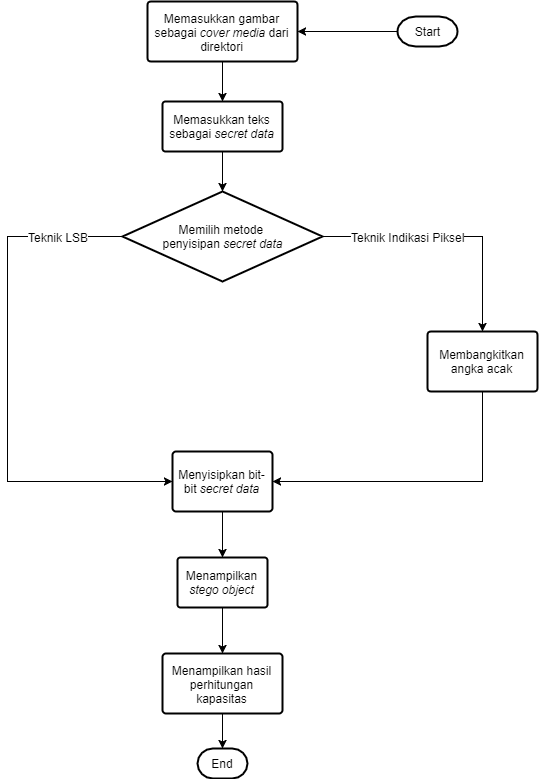
\includegraphics[scale=0.5]{Construct.png}
		\caption{\textit{Flowchart} proses implementasi steganografi pada perangkat lunak}
		\label{imageCons}
		\end{figure}		
		
		Ekstraksi \textit{secret data} dapat dilakukan setelah mendapatkan \textit{stego object} hasil implementasi steganografi dengan salah satu dari kedua metode. Perangkat lunak membutuhkan masukan berupa gambar yang ingin diekstraksi. Gambar tersebut harus merupakan hasil implementasi salah satu metode steganografi. Apabila gambar tersebut merupakan hasil implementasi LSB, maka ekstraksi harus dilakukan dengan metode LSB. Apabila gambar tersebut merupakan hasil implementasi teknik indikasi piksel, maka ekstraksi harus dilakukan dengan teknik indikasi piksel. Perangkat lunak terlebih dahulu harus mengekstraksi nilai-nilai \textit{channel} warna pada setiap piksel gambar \textit{stego object}. Nilai-nilai \textit{channel} warna akan diubah ke dalam bentuk  8 bit angka biner.\\
		
		Apabila ekstraksi dilakukan dengan metode LSB, perangkat lunak akan menelusuri piksel-piksel pada \textit{stego object} dan menyimpan bit-bit terakhir pada setiap nilai \textit{channel} warna dalam bentuk biner. Bit-bit tersebut akan disimpan dan nantinya diubah ke dalam bentuk teks berdasarkan kode ASCII. Perangkat lunak akan menampilkan \textit{secret data} hasil ekstraksi dalam bentuk teks.\\
		
		Apabila ekstraksi dilakukan dengan teknik indikasi piksel dengan modifikasi, maka perangkat lunak akan meminta pengguna memasukkan angka yang menentukan baris piksel awal yang ingin ditelusuri. Selain itu, perangkat lunak juga akan meminta masukan berupa panjang karakter \textit{secret data}. Perangkat lunak kemudian akan menentukan \textit{channel} yang menjadi indikator, \textit{channel} 1, dan \textit{channel} 2. Bit-bit \textit{secret data} akan disimpan berdasarkan nilai \textit{channel} yang menjadi indikator pada setiap baris piksel. Bit-bit \textit{secret data} akan diubah ke dalam bentuk teks berdasarkan kode ASCII. Perangkat lunak akan menampilkan \textit{secret data} hasil ekstraksi dalam bentuk teks. Gambar \ref{imageRecons} menunjukkan aliran proses ekstraksi \textit{secret data} dengan teknik LSB dan teknik indikasi piksel pada perangkat lunak.\\
		
		\begin{figure}[!htbp]
		\centering
		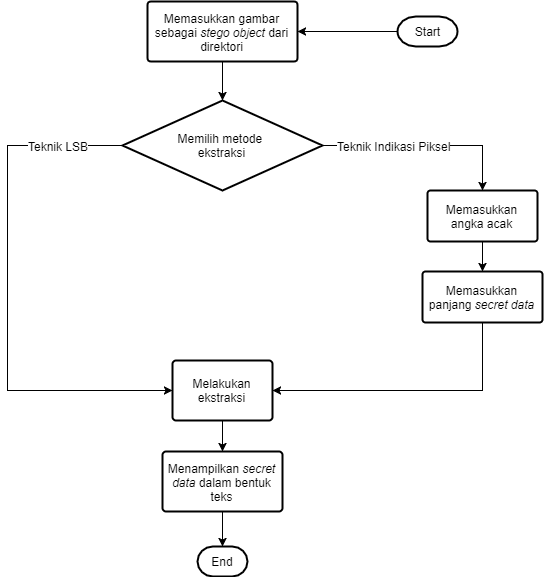
\includegraphics[scale=0.5]{Reconstruct.png}
		\caption{\textit{Flowchart} proses ekstraksi pada perangkat lunak}
		\label{imageRecons}
		\end{figure}
		
		Berikut merupakan deskripsi setiap langkah proses ekstraksi \textit{secret data} yang terdapat pada Gambar \ref{imageRecons}.
		
		\begin{itemize}
		\item Memilih gambar dari direktori\\
		Pengguna memilih gambar dari direktori untuk dilakukan ekstraksi.
		\item Memilih metode ekstraksi\\
		Pengguna memilih apakah metode LSB atau teknik indikasi piksel yang akan digunakan untuk melakukan  ekstraksi.
		\item Memasukkan angka acak\\
		Apabila memilih metode teknik indikasi piksel, maka pengguna harus memasukkan angka yang menyatakan baris piksel awal dilakukan ekstraksi. Angka ini didapatkan dari hasil pembangkitan angka acak pada proses implementasi steganografi.
		\item Memasukkan panjang \textit{secret data}\\
		Selain memasukkan angka acak, pengguna juga harus memasukkan panjang \textit{secret data} yang merupakan salah satu kunci untuk melakukan ekstraksi. Melalui panjang \textit{secret data}, perangkat lunak dapat menentukan \textit{channel} warna yang menjadi indikator, \textit{channel} 1, dan \textit{channel} 2.
		\item Melakukan ekstraksi\\
		Perangkat lunak melakukan ekstraksi terhadap gambar untuk mendapatkan bit \textit{secret data} dengan menggunakan metode yang sudah dipilih.
		\item Menampilkan \textit{secret data} berupa teks\\
		Perangkat lunak menyimpan bit-bit \textit{secret data} hasil ekstraksi gambar, kemudian menampilkannya setelah diubah dalam bentuk teks.
		\end{itemize}
				
				
		\item \textbf{Melakukan perancangan perangkat lunak}\\
		{\bf Status :} Ada sejak rencana kerja skripsi.\\
		{\bf Hasil :} Perancangan perangkat lunak yang diselesaikan pada skripsi 1 adalah diagram kelas awal. Berikut merupakan hasil perancangan perangkat lunak yang diselesaikan pada skripsi 1.\\
		
		\textbf{Diagram Kelas Awal}\\
		Diagram kelas awal merupakan gambaran rancangan awal hubungan antara kelas satu dan lainnya yang digunakan untuk membangun perangkat lunak. Gambar \ref{imageClassDiagram} menunjukkan bahwa kelas yang akan digunakan berjumlah 4 kelas. Berikut merupakan rincian kelas beserta atribut-atributnya.\\
		
		\begin{figure}[!htbp]
		\centering
		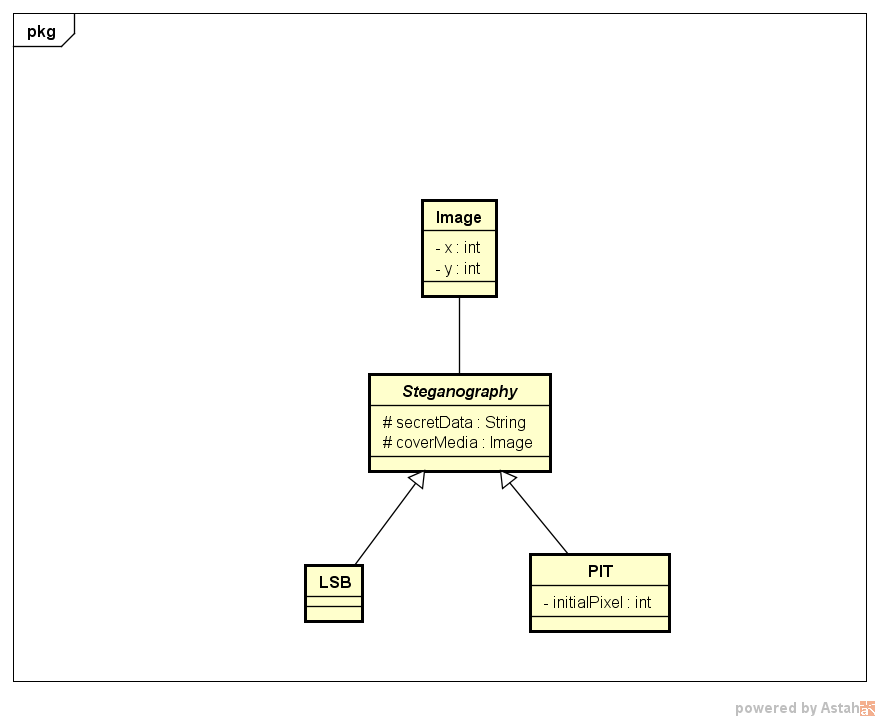
\includegraphics[scale=0.4]{ClassDiagram.png}
		\caption{Diagram kelas awal}
		\label{imageClassDiagram}
		\end{figure}
		
		\begin{enumerate}
			\item Kelas Image\\
			Kelas Image merepresentasikan \textit{cover media} yang digunakan pada penyisipan bit \textit{secret data}. Kelas ini membantu kelas Steganography untuk mengakses nilai-nilai piksel pada \textit{cover media}. Kelas Image memiliki dua buah atribut, antara lain:
			\begin{itemize}
				\item Atribut x : Atribut x merepresentasikan nilai absis dalam koordinat letak piksel pada gambar. 
				\item Atribut y : Atribut y merepresentasikan nilai ordinat dalam koordinat letak piksel pada gambar.
			\end{itemize}
			\item Kelas Steganography\\
			Kelas Steganography merupakan kelas utama yang mengimplementasikan metode penyisipan bit. Kelas ini bertipe abstrak dan memiliki dua \textit{subclass},yaitu kelas LSB dan kelas PIT. Kelas Steganography memiliki dua atribut, antara lain:
			\begin{itemize}
				\item Atribut secretData : Atribut secretData merepresentasikan \textit{secret data} yang akan disembunyikan dalam tipe String.
				\item Atribut coverMedia : Atribut coverMedia merepresentasikan \textit{cover media} yang akan digunakan untuk menyembunyikan \textit{secret data} dalam tipe Image.
			\end{itemize}
			\item Kelas LSB\\
			Kelas LSB merupakan kelas turunan dari kelas Steganography yang akan mengimplementasikan penyisipan bit \textit{secret data} pada \textit{cover media} dengan metode LSB.
			\item Kelas PIT\\
			Kelas PIT merupakan kelas turunan dari kelas Steganography yang akan mengimplementasikan penyisipan bit \textit{secret data} pada \textit{cover media} dengan teknik indikasi piksel.
		\end{enumerate}

		\item \textbf{Mengimplementasikan teknik indikasi piksel dan algoritma \textit{Triple-A} pada perangkat lunak}\\
		{\bf Status :} Diganti (metode \textit{Triple-A} diganti menjadi metode \textit{Least Significant Bit}).\\
		{\bf Hasil :}

		\item \textbf{Melakukan pengujian teknik indikasi piksel dan algoritma \textit{Triple-A}}\\
		{\bf Status :} Diganti (metode \textit{Triple-A} diganti menjadi metode \textit{Least Significant Bit}). \\
		{\bf Hasil :} 

		\item \textbf{Melakukan analisis terhadap hasil pengujian} \\
		{\bf Status :} Ada sejak rencana kerja skripsi.\\
		{\bf Hasil :}

		\item \textbf{Menulis dokumen skripsi}\\
		{\bf Status :} Ada sejak rencana kerja skripsi.\\
		{\bf Hasil :} 	

	\end{enumerate}

\section{Pencapaian Rencana Kerja}
Persentase penyelesaian skripsi sampai dengan dokumen ini dibuat dapat dilihat pada tabel berikut :

\begin{center}
  \begin{tabular}{ | c | c | c | c | l | c |}
    \hline
    1*  & 2*(\%) & 3*(\%) & 4*(\%) &5* & 6*(\%) \\ \hline \hline
    1   & 15 & 15 &  &  & 15 \\ \hline
    2   & 5 & 5 &  &  & 5 \\ \hline
    3   & 10 & 10 &  &  & 10 \\ \hline
    4   & 10 & 5 & 5 & {\footnotesize Diagram kelas awal dikerjakan pada skripsi 1.} & 5 \\ \hline
    5   & 25 &  & 25 & & \\ \hline
    6   & 10 &  & 10 & & \\ \hline
    7   & 5 &  & 5 & & \\ \hline    
    8	& 20 & 5 & 15 & {\footnotesize Pendahuluan, dasar teori, dan analisis dikerjakan pada skripsi 1.} &  5 \\ \hline
    Total  & 100  & 40  & 60 &  & 40 \\ \hline
	\end{tabular}
\end{center}

Keterangan (*)\\
1 : Bagian pengerjaan Skripsi (nomor disesuaikan dengan detail pengerjaan di bagian 5)\\
2 : Persentase total \\
3 : Persentase yang akan diselesaikan di Skripsi 1 \\
4 : Persentase yang akan diselesaikan di Skripsi 2 \\
5 : Penjelasan singkat apa yang dilakukan di S1 (Skripsi 1) atau S2 (skripsi 2)\\
6 : Persentase yang sidah diselesaikan sampai saat ini 

%\section{Kendala yang dihadapi}
%TULISKAN BAGIAN INI JIKA DOKUMEN ANDA TIPE A ATAU C

\newpage
\vspace{1cm}
\centering Bandung, \tanggal\\
\vspace{2cm} \nama \\ 
\vspace{1cm}

Menyetujui, \\
\ifdefstring{\jumpemb}{2}{
\vspace{1.5cm}
\begin{centering} Menyetujui,\\ \end{centering} \vspace{0.75cm}
\begin{minipage}[b]{0.45\linewidth}
% \centering Bandung, \makebox[0.5cm]{\hrulefill}/\makebox[0.5cm]{\hrulefill}/2013 \\
\vspace{2cm} Nama: \pembA \\ Pembimbing Utama
\end{minipage} \hspace{0.5cm}
\begin{minipage}[b]{0.45\linewidth}
% \centering Bandung, \makebox[0.5cm]{\hrulefill}/\makebox[0.5cm]{\hrulefill}/2013\\
\vspace{2cm} Nama: \pemB \\ Pembimbing Pendamping
\end{minipage}
\vspace{0.5cm}
}{
% \centering Bandung, \makebox[0.5cm]{\hrulefill}/\makebox[0.5cm]{\hrulefill}/2013\\
\vspace{2cm} Nama: \pembA \\ Pembimbing Tunggal
}
\end{document}

